%% Please change the file name by replacing N with the apporpriate number
%% corresponding to the current homework and XX with your initials.
%% https://www.math.uci.edu/~gpatrick/jsOnline/hw1.html

\documentclass{beamer}
\usepackage{amssymb,amsfonts,color,graphicx,amsmath,enumerate}
\usepackage{tikz} %This package offers the ability to draw pictures
\usepackage{amsthm}

\newcommand{\naturals}{\mathbb{N}}
\newcommand{\integers}{\mathbb{Z}}
\newcommand{\complex}{\mathbb{C}}
\newcommand{\reals}{\mathbb{R}}
\newcommand{\exreals}{\overline{\mathbb{R}}}
\newcommand{\mcal}[1]{\mathcal{#1}}
\newcommand{\mable}{measurable}
\newcommand{\quats}{\mathbb{H}}
\newcommand{\rationals}{\mathbb{Q}}
\newcommand{\norm}{\trianglelefteq}
\newcommand{\Aut}{\text{Aut}}
\newcommand{\disk}{\mathbb{D}}
\newcommand{\halfplane}{\mathbb{H}}
\newcommand{\Lp}[2]{\left\|{#1}\right\|_{L^{#2}}}
\newcommand{\supp}[1]{\text{supp}({#1})}
\newcommand{\Hom}[2]{\text{Hom}_{{#1}}({#2})}
\newcommand{\tr}{\text{tr}}
\newcommand{\field}[1]{\mathbb{F}_{{#1}}}
\newcommand{\Gal}[1]{\text{Gal}\left({#1}\right)}
\newcommand{\esssup}{\text{ess sup }}
\newcommand{\essinf}{\text{ess inf }}
\newcommand{\affine}{\mathbb{A}}

%\newenvironment{solution}
%{\begin{proof}[Solution]}
%{\end{proof}}

\title{Secret Sharing}
\author{Liam Hardiman}

\usetheme{Frankfurt}

\begin{document}

\maketitle

\begin{frame}
	\frametitle{What is Secret Sharing?}
	\begin{itemize}
		\item Eleven scientists are working on a secret project. They wish to lock up the documents in a cabinet so that the cabinet can be opened if and only if six or more of the scientists are present. What is the smallest number of locks needed? What is the smallest number of keys to the locks each scientist must carry?\footnote{Liu, C.L \textit{Introduction to Combinatorial Mathematics}. McGraw-Hill, New York, 1968}\\\pause

		\item $\binom{11}{6} = 462$ locks and $\binom{10}{5} = 252$ keys.
	\end{itemize}
\end{frame}

\begin{frame}
	\frametitle{What is Secret Sharing?}

	The goal of secret sharing is dividing a secret $S$ into $n$ pieces, called \textit{shares}, so that no fewer than $k\leq n$ shares are sufficient for reassembling $S$. This is called a $(k,n)$\textbf{-threshold scheme}.
\end{frame}

\begin{frame}
	\frametitle{Why is Secret Sharing?}
	``Threshold schemes are ideally suited to applications in which a group of mutually suspicious individuals with conflicting interests must cooperate.'' -- Adi Shamir
\end{frame}

\begin{frame}
	\frametitle{Example Application}
	\begin{itemize}
		\item Imagine a company stamps its checks with a digital signature\pause
		\item Risky to give the signing key to every low-level executive\pause
	\end{itemize}
	\vspace{1cm}
	\centering
	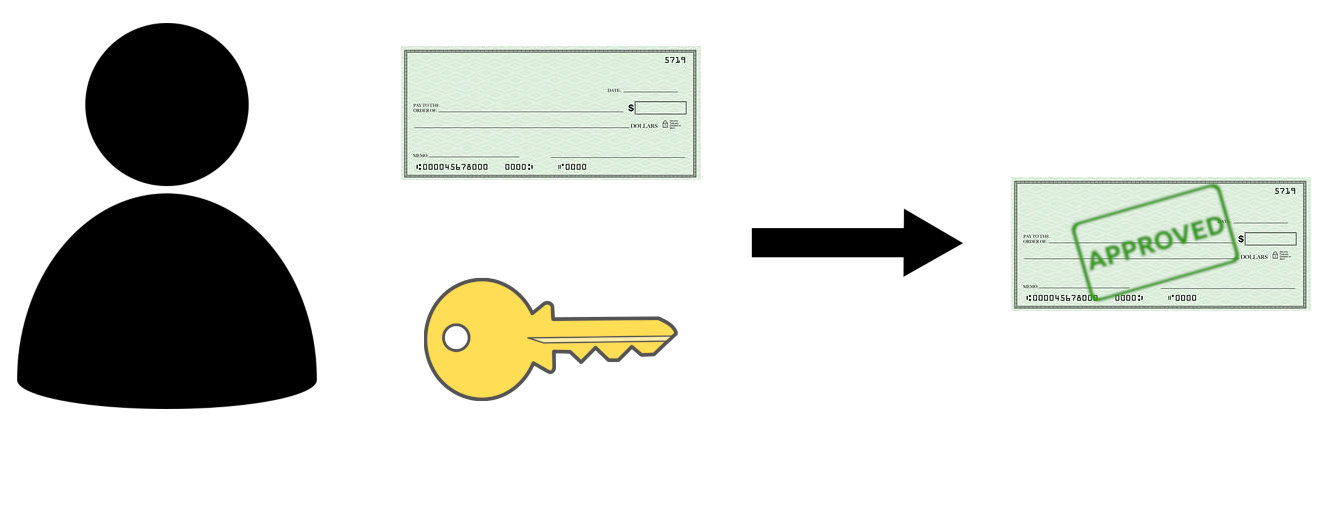
\includegraphics[scale=.6]{one_exec.png}
\end{frame}

\begin{frame}
	\frametitle{Example Application}
	\begin{itemize}
		\item Set up an $(n,3)$-threshold scheme for the key\pause
		\item Give each executive a key fragment card and a check signing machine\pause
	\end{itemize}
	\vspace{1cm}
	\centering
	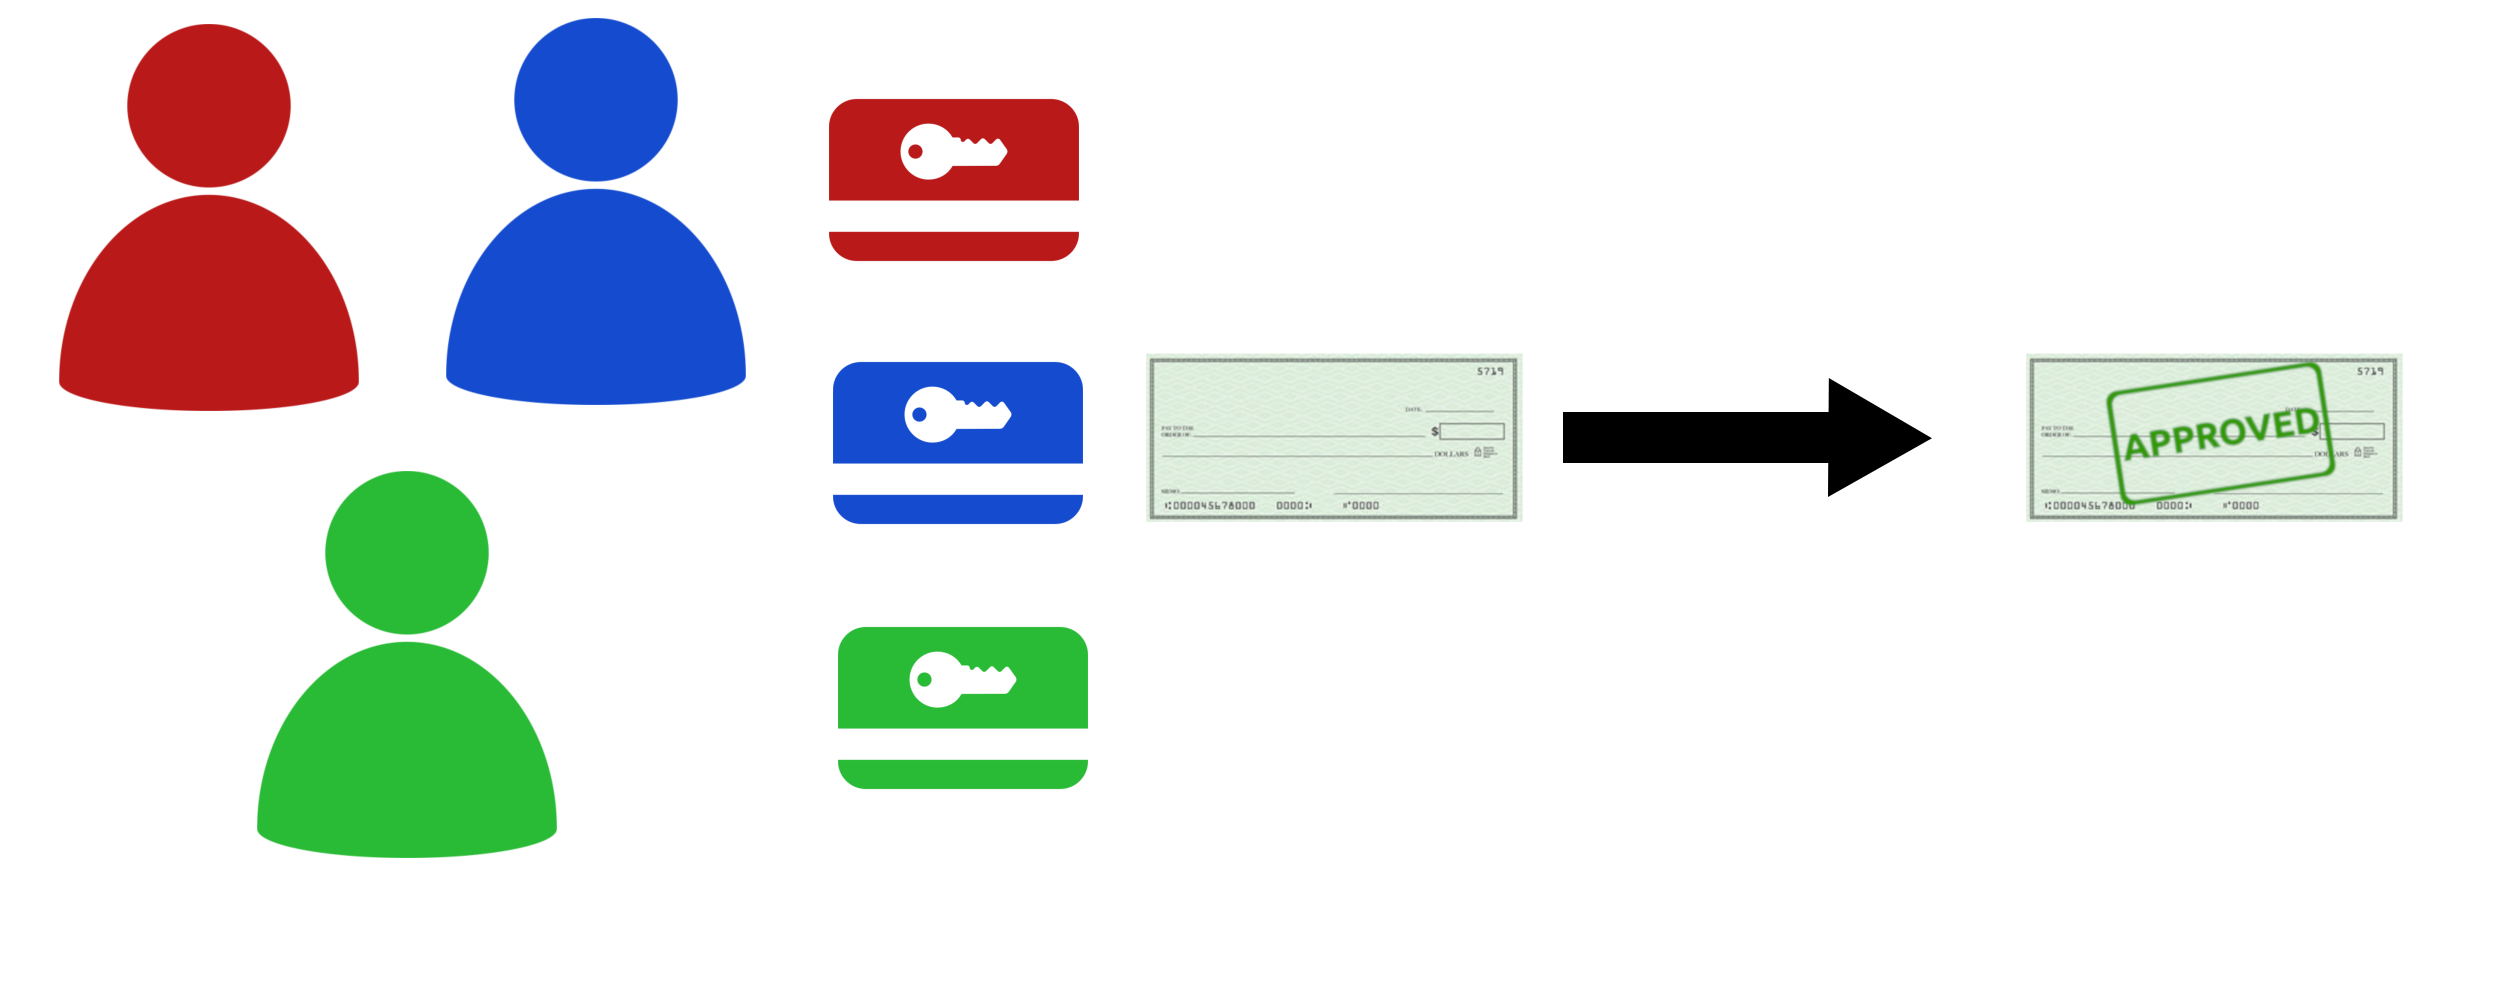
\includegraphics[scale=.3]{three_execs.png}
\end{frame}

\begin{frame}
	\frametitle{Example Application}
	\begin{itemize}
		\item This solution is flexible\pause
	\end{itemize}
	\vspace{1cm}
	\centering
	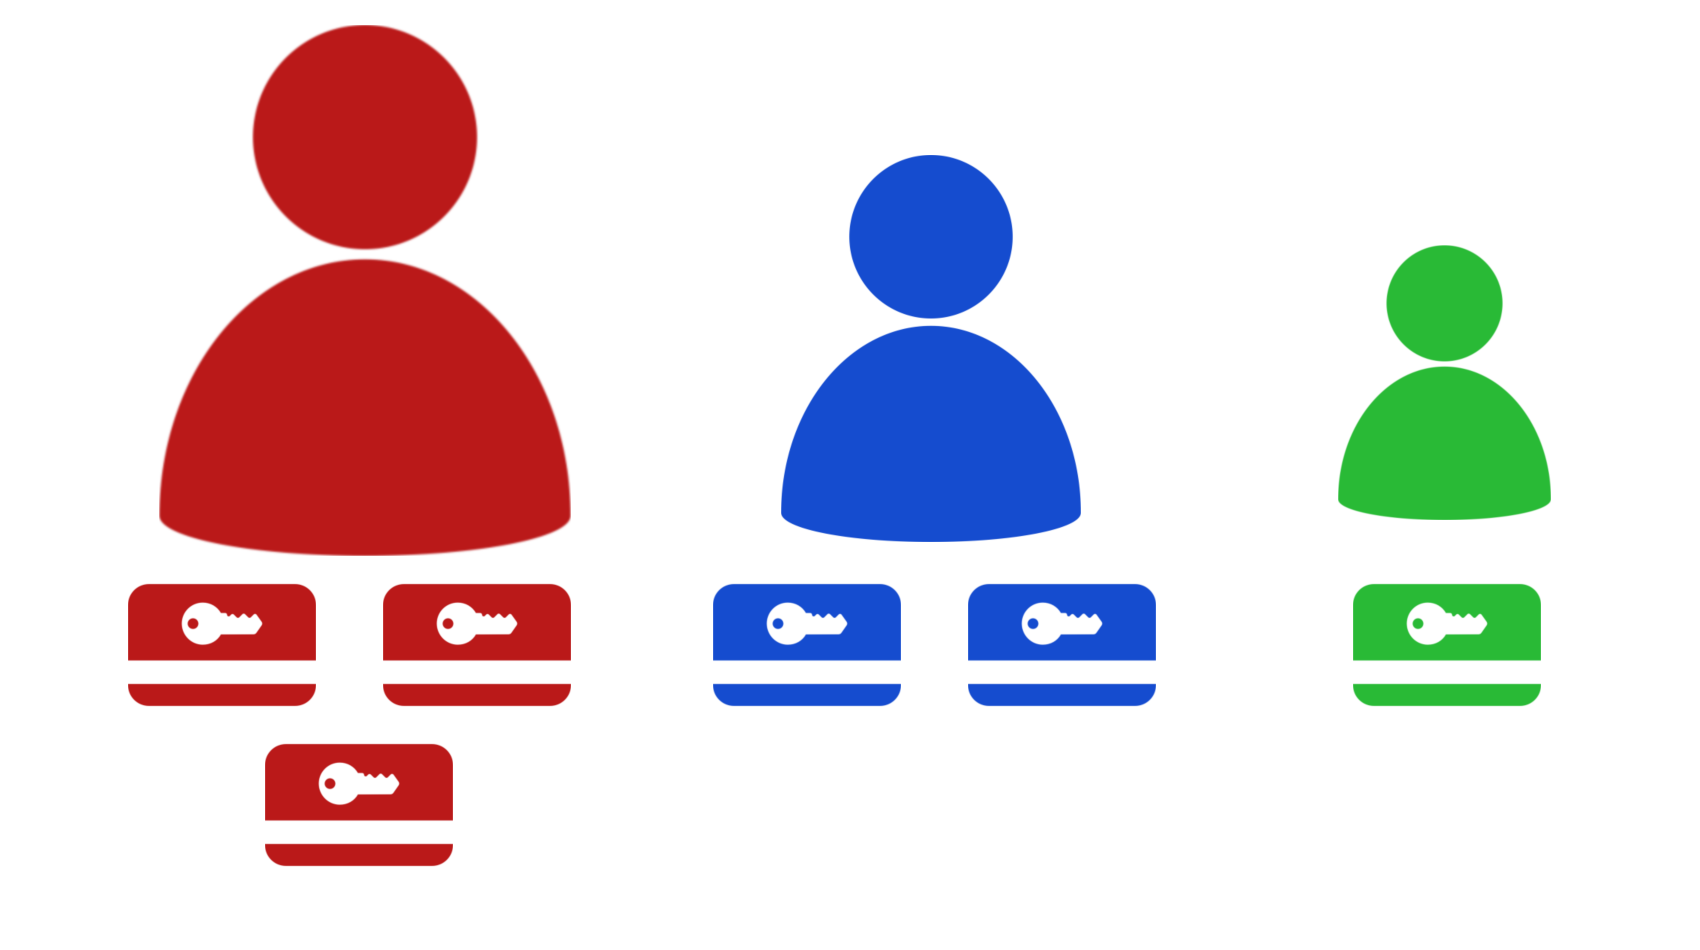
\includegraphics[scale=.2]{exec_levels.png}
\end{frame}

\begin{frame}
	\frametitle{How is Secret Sharing? - Shamir's Method (1979)\footnote{A. Shamir, ``How to share a secret''. Commun. ACM 22(11), 612–613 (1979)}}
	\begin{itemize}
		\item Say we want to set up a $(k,n)$-threshold scheme\pause
		\item Choose a big prime $p$ and let the secret, $S$, be an element in $\integers/p\integers$\pause
		\item Choose random elements $a_1, \ldots, a_{k-1}\in \integers/p\integers$. Set
		\[
		p(x) = S + a_1x + \cdots + a_{k-1}x^{k-1}.
		\]\pause
		\item Issue to person $i$, $1\leq i\leq n$, the share $D_i = (i, p(i))$.
	\end{itemize}
\end{frame}

\begin{frame}
	\frametitle{How is Secret Sharing? - Shamir's Method (1979)}
	\begin{itemize}
		\item $m$ shares, $D_1,\ldots, D_m$, give us $m$ linear equations in $k$ unknowns\pause
		\[
			\begin{array}{ccccccccccc}
				S & + & a_1\cdot 1  &+& \cdots& + & a_{k-1}(1)^{k-1} & = & p(1)\\
				S & + & a_2\cdot 2  &+& \cdots& + & a_{k-1}(2)^{k-1} & = & p(2)\\
				&&&&&&\vdots&&&\\
				S & + & a_1\cdot m &+& \cdots& + & a_{k-1}(m)^{k-1} & = & p(m)
			\end{array}
		\]
		\item Linear algebra tells us we get a solution if and only if we have at least $k$ equations (shares)
	\end{itemize}
\end{frame}

\begin{frame}
	\frametitle{Downside to Shamir's Scheme}
	Each share is an element of $\integers/p\integers$, just like the secret. $n$ shares means $n$ times the storage.
\end{frame}

\begin{frame}
	\frametitle{Information Dispersal - Rabin (1989)\footnote{M. O. Rabin, ``Efficient Dispersal of Information for Security, Load Balancing, and Fault Tolerance''. In: Journal of the ACM, vol. 36, iss. 2, 1989, pp. 335-348}}
	
	\begin{itemize}
		\item Split a file $F$ into $n$ pieces so that any $k\leq n$ pieces can reconstruct $F$\pause
		\item Each piece has size roughly $|F|/k$. That means roughly $n/k$ blowup, which can be close to unity\pause
		\item Not perfectly secret
	\end{itemize}	
\end{frame}

\begin{frame}
	\frametitle{Information Dispersal - Rabin (1989)}

	\begin{itemize}
		\item Split the 800 byte file, $F = b_1, \ldots, b_{800}$, among 15 people so that any 8 of them can reassemble it. Each $b_i$ is an integer between 0 and 255\pause
		\item Break the file into 8 byte blocks
		\begin{align*}
		F &= (b_1, \ldots, b_8), (b_9, \ldots, b_{16}), \ldots, (b_{793}, \ldots, b_{800})\\
		&= f_1, f_2, \ldots, f_{100}
		\end{align*}\pause
	\end{itemize}

\end{frame}

\begin{frame}
	\frametitle{Information Dispersal - Rabin (1989)}
	\begin{itemize}
		\item To create 15 shares, choose 15 vectors, $a_j$, $1\leq j\leq 15$ in $(\integers/p\integers)^8$ so that any 8 different vectors is linearly independent\pause

		\item To compute the $j$-th share, we compress each block of $F$ by calculating the dot product $F_{ji} = a_j\cdot f_i\pmod{p}$ for each $1\leq i\leq 100$.\pause
	\end{itemize}
	\vspace{.5cm}
	\centering
	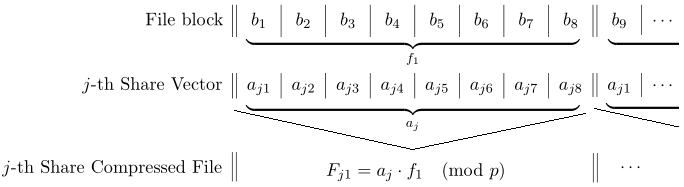
\includegraphics[scale=.5]{rabin_compression.png}
\end{frame}

\begin{frame}
	\frametitle{Information Dispersal - Rabin (1989)}
	\begin{itemize}
		\item This gives a compressed file $F_j = F_{j1}, \ldots, F_{j(100)}$. Let the $j$-th share be $S_j = (a_j, F_j)$, $1\leq j\leq 15$.\pause
		\item If we're given 8 shares we get this matrix equation
		\[
		\begin{bmatrix}
			\text{---} & a_1 & \text{---}\\
			&\vdots&\\
			\text{---} & a_8 & \text{---}
		\end{bmatrix}
		\begin{bmatrix}
			b_1\\
			\vdots\\
			b_8
		\end{bmatrix}=
		\begin{bmatrix}
			F_{1,1}\\
			\vdots\\
			F_{8,1}
		\end{bmatrix}.
		\]\pause
		\item With 8 shares, this matrix is invertible and we can recover the first block. The same matrix recovers all blocks
	\end{itemize}
\end{frame}

\begin{frame}
	\frametitle{Secret Sharing with Short Shares - Krawczyk (1994)\footnote{H. Krawczyk, ``Secret Sharing Made Short''. In: Stinson D.R. (eds) Advances in Cryptology — CRYPTO’ 93. CRYPTO 1993. Lecture Notes in Computer Science, vol 773.}}
	\begin{itemize}
		\item Let's set up a $(k,n)$-threshold scheme\pause
		\item Encrypt $S$ with some secure cipher using key $K$, $E = Enc(S,K)$\pause
		\item Use Rabin's information dispersal to split $E$ into $n$ pieces, each with size $\frac{n}{k}\cdot |E|$\pause
		\item Use Shamir's secret sharing to split $K$ into $n$ pieces, each with size $|K|$
	\end{itemize}
\end{frame}

\end{document}